%!TEX program = xelatex
\documentclass[dvipsnames, svgnames,a4paper,11pt]{article}
% ----------------------------------------------------- 
%	加边框的命令
%	参考:https://tex.stackexchange.com/questions/531559/how-to-add-the-page-border-for-first-two-pages-in-latex
\usepackage{tikz}
\usetikzlibrary{calc}
\usepackage{eso-pic}
\AddToShipoutPictureBG{%
\begin{tikzpicture}[overlay,remember picture]
\draw[line width=0.6pt] % 边框粗细
    ($ (current page.north west) + (0.6cm,-0.6cm) $)
    rectangle
    ($ (current page.south east) + (-0.6cm,0.6cm) $); % 边框位置
\end{tikzpicture}}


\usepackage{xcolor}
\definecolor{c1}{HTML}{086173} % 目录颜色 原版为2752C9 紫灰色535AAA 蓝紫色0B0DB7 深蓝色070F94 湖绿色219394 松石灰绿086173
\definecolor{c2}{HTML}{E20129} % 引用颜色 原版\definecolor{c2}{RGB}{190,20,83} 橙色F24729

\usepackage{ctex}
\usepackage[top=28mm,bottom=28mm,left=15mm,right=15mm]{geometry}
\usepackage{hyperref} 
\hypersetup{
	colorlinks,
	linktoc = section, % 超链接位置,选项有section, page, all
	linkcolor = c1, % linkcolor 目录颜色
	citecolor = c1  % citecolor 引用颜色
}
\usepackage{amsmath,enumerate,multirow,float}
\usepackage{tabularx}
\usepackage{tabu}
\usepackage{subfig}
\usepackage{fancyhdr}
\usepackage{graphicx}
\usepackage{wrapfig}  
\usepackage{physics}
\usepackage{appendix}
\usepackage{amsfonts}

%
\usepackage{tcolorbox}
\tcbuselibrary{skins,breakable}
\newtcolorbox{tbox}[2][]{
    colframe=black!70!,
    breakable,
    enhanced,
	boxrule =0.5pt,
    title = {#2},
    fonttitle = \large\kaishu\bfseries,
	drop fuzzy shadow,
    #1
}
\newtcolorbox[auto counter,number within=section]{question}[1][]{
  top=2pt,bottom=2pt,arc=1mm,
  boxrule=0.5pt,
%   frame hidden,
  breakable,
  enhanced, %跨页后不会显示下边框
  coltitle=c1!80!gray,
  colframe=c1,
  colback=c1!3!white,
  drop fuzzy shadow,
  title={思考题~\thetcbcounter:\quad},
  fonttitle=\bfseries,
  attach title to upper,
  #1
}

% ---------------------------------------------------------------------
%	利用cleveref改变引用格式,\cref是引用命令
\usepackage{cleveref}
\crefformat{figure}{#2{\textcolor{c2}{Figure #1}}#3} % 图片的引用格式
\crefformat{equation}{#2{(\textcolor{c2}{#1})}#3} % 公式的引用格式
\crefformat{table}{#2{\textcolor{c2}{Table #1}}#3} % 表格的引用格式


% ---------------------------------------------------------------------
%	页眉页脚设置
\fancypagestyle{plain}{\pagestyle{fancy}}
\pagestyle{fancy}
\lhead{\kaishu 中山大学物理与天文学院电子技术实验\uppercase\expandafter{\romannumeral1}} % 左边页眉,学院 + 课程
\rhead{\kaishu 实验报告By黄罗琳} % 右边页眉,实验报告标题
\cfoot{\thepage} % 页脚,中间添加页码


% ---------------------------------------------------------------------
%	对目录、章节标题的设置
\renewcommand{\contentsname}{\centerline{\huge 目录}}
\usepackage{titlesec}
\usepackage{titletoc}
% \titleformat{章节}[形状]{格式}{标题序号}{序号与标题间距}{标题前命令}[标题后命令]
\titleformat{\section}{\centering\LARGE\songti}{}{1em}{}

% ---------------------------------------------------------------------
%   listing代码环境设置
\usepackage{listings}
\lstloadlanguages{python}
\lstdefinestyle{pythonstyle}{
backgroundcolor=\color{gray!5},
language=python,
frameround=tftt,
frame=shadowbox, 
keepspaces=true,
breaklines,
columns=spaceflexible,                   
basicstyle=\ttfamily\small, % 基本文本设置,字体为teletype,大小为scriptsize
keywordstyle=[1]\color{c1}\bfseries, 
keywordstyle=[2]\color{Red!70!black},   
stringstyle=\color{Purple},       
showstringspaces=false,
commentstyle=\ttfamily\scriptsize\color{green!40!black},%注释文本设置,字体为sf,大小为smaller
tabsize=2,
morekeywords={as},
morekeywords=[2]{np, plt, sp},
numbers=left, % 代码行数
numberstyle=\it\tiny\color{gray}, % 代码行数的数字字体设置
stepnumber=1,
rulesepcolor=\color{gray!30!white}
}




% ---------------------------------------------------------------------
%	其他设置
\def\degree{${}^{\circ}$} % 角度
\graphicspath{{./images/}} % 插入图片的相对路径
\allowdisplaybreaks[4]  %允许公式跨页 
\usepackage{lipsum}
\usepackage{adjustbox}
%\usepackage{mathrsfs} % 字体
%\captionsetup[figure]{name=Figure} % 图片形式
%\captionsetup[table]{name=Table} % 表格形式
\begin{document}
	
	% 实验报告封面	
	% 顶栏
	\begin{table}
		\renewcommand\arraystretch{1.7}
		\begin{tabularx}{\textwidth}{
				|X|X|X|X
				|X|X|X|X|}
			\hline
			\multicolumn{2}{|c|}{预习报告}&\multicolumn{2}{|c|}{实验记录}&\multicolumn{2}{|c|}{分析讨论}&\multicolumn{2}{|c|}{总成绩}\\
			\hline
			\LARGE25 & & \LARGE25 & & \LARGE30 & & \LARGE80 & \\
			\hline
		\end{tabularx}
	\end{table}
	% ---
	
	% 信息栏
	\begin{table}
		\renewcommand\arraystretch{1.7}
		\begin{tabularx}{\textwidth}{|X|X|X|X|}
			\hline
			年级、专业: & 2022级 物理学 &组号: & D8\\
			\hline
			姓名: & 黄罗琳、王显   & 学号: &22344001、22344002   \\
			\hline
			实验时间: & 2024/4/24 & 教师签名: & \\
			\hline
		\end{tabularx}
	\end{table}
	% ---
	
	% 大标题
	\begin{center}
		\LARGE ET8 \quad 单级交流放大器
	\end{center}
	% ---
	
	% 注意事项
	
	% 基本
	\textbf{【实验报告注意事项】}
	\begin{enumerate}
		\item 实验报告由三部分组成:
		\begin{enumerate}
			\item 预习报告:课前认真研读实验讲义,弄清实验原理;实验所需的仪器设备、用具及其使用、完成课前预习思考题;了解实验需要测量的物理量,并根据要求提前准备实验记录表格(可以参考实验报告模板,可以打印)。\textcolor{red}{\textbf{(20分)}}
			\item 实验记录:认真、客观记录实验条件、实验过程中的现象以及数据。实验记录请用珠笔或者钢笔书写并签名(\textcolor{red}{\textbf{用铅笔记录的被认为无效}})。\textcolor{red}{\textbf{保持原始记录,包括写错删除部分,如因误记需要修改记录,必须按规范修改。}}(不得输入电脑打印,但可扫描手记后打印扫描件);离开前请实验教师检查记录并签名。\textcolor{red}{\textbf{(30分)}}
			\item 数据处理及分析讨论:处理实验原始数据(学习仪器使用类型的实验除外),对数据的可靠性和合理性进行分析;按规范呈现数据和结果(图、表),包括数据、图表按顺序编号及其引用;分析物理现象(含回答实验思考题,写出问题思考过程,必要时按规范引用数据);最后得出结论。\textcolor{red}{\textbf{(30分)}}
		\end{enumerate}
		\textbf{实验报告就是将预习报告、实验记录、和数据处理与分析合起来,加上本页封面。\textcolor{red}{(80分)}}
	
\end{enumerate}
	
	% 目录
	\clearpage
	\tableofcontents
	\clearpage
	% ---
	
	
	
	% 预习报告	
	
	% 小标题
	\setcounter{section}{0}
	\section{ET8 单级交流放大器\quad\heiti 预习报告}
	% ---
	
	% 实验目的
	\subsection{实验目的}
	\begin{enumerate}
		\item 掌握放大电路静态工作点的测试方法,进一步理解电路元件参数对静态工作点的影响,以及调整静态工作点的方法。
		\item 掌握测量电压放大倍数、输入电阻、输出电阻及最大不失真输出电压幅值的方法。
		\item 观察电路参数对失真的影响。
	\end{enumerate}
	% ---
	
	% 仪器用具
	\subsection{仪器用具}
	\begin{table}[htbp]
		\centering
		\renewcommand\arraystretch{1.6}
		\begin{tabular}{p{0.05\textwidth}|p{0.20\textwidth}|p{0.05\textwidth}|p{0.5\textwidth}}
			\hline
			编号 & 仪器用具名称 & 数量 & 主要参数(型号,测量范围,测量精度等) \\
			\hline
			1 & 实验箱 & 1 & \\
			\hline
			2 & 数字万用表 & 1 &  \\
			\hline
			3 & 函数信号发生器 & 1 & \\
			\hline
			4 & 交流毫伏表 & 1 &  \\
			\hline
			5 & 双踪示波器 & 1 & \\
			\hline
		\end{tabular}
	\end{table}
	
	% ---

	
	
	% 原理概述
	\subsection{原理概述}
	\begin{enumerate}
		\item 静态工作点
		\begin{figure}[{H}]
			\centering
			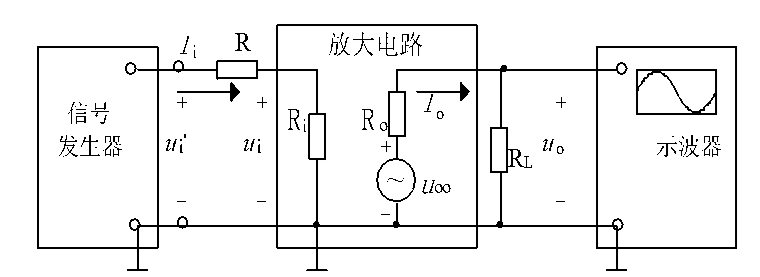
\includegraphics[width=0.6\linewidth]{交流放大电路.png}
			\caption{交流放大电路实验电路图}
			\label{}
		\end{figure}

		 放大电路的静态工作点决定了电路在没有输入信号时的电流和电压状态,这对于放大器的性能和稳定性至关重要。选择合适的静态工作点需要了解晶体管的特性、确定目标工作范围、选择合适的偏置电路,并进行必要的计算和测试。测试后,还需根据实际结果调整偏置参数,确保放大器在线性区域内稳定运行,避免失真,并考虑温度等外部因素对工作点的影响。通过这些步骤,可以确保放大器在各种条件下稳定运行,获得良好的增益和频率响应。
		
		静态工作点的选取十分重要,它影响放大器的放大倍数、波形失真及工作稳定性等。静态工作点如果选择不当会产生饱和失真或截止失真。一般情况下,调整静态工作点,就是调整电路有关电阳, 使$I_{co}$和$U_{CEO}$达到合适的值。
		\item 放大电路的基本性能及测量方法
		\begin{enumerate}
\item \textbf{电压放大倍数 $A_u$}

电压放大倍数 $A_u$ 是放大电路电压放大能力的一个指标,定义为输出电压幅值与输入电压幅值的比率。这一指标也被称作增益,其公式为:
$$A_u = \frac{U_o}{U_i}$$
要获得电压放大倍数 $A_u$,可以使用晶体管毫伏表测量 $U_o$ 和 $U_i$。

\item \textbf{输入电阻 $R_i$}

输入电阻 $R_i$ 表示放大电路从前一级获取电流的能力。放大器的输入电阻是从放大器输入端看进去的等效电阻。公式表示如下:
$$R_i = \frac{U_i}{I_i}$$
一种测量输入电阻的方法是在放大器的输入端串联一个已知电阻 $R$,建议选择 $R$ 大致等于估算的输入电阻。在不失真的情况下,使用晶体管毫伏表测量电阻 $R$ 两端对地的电压 $U_i'$ 以及输入电压 $U_i$。此时,输入电阻的计算公式为:
$$R_i = \frac{U_i}{U_i' - U_i} \cdot R$$

\item \textbf{输出电阻 $R_o$}

输出电阻 $R_o$ 是从放大电路输出端看进去的等效电阻。定义为输出电压与输出电流的比率。具体计算方法是:在输入端施加信号,在不失真的情况下,使用晶体管毫伏表分别测量放大器空载和带负载时的输出电压 $U_{\infty}$ 和 $U_{oL}$,那么输出电阻可以计算为:
$$R_o = \frac{U_{\infty} - U_{oL}}{I_o} = \frac{U_{\infty} - U_{oL}}{U_{oL}} \cdot R_L$$


\end{enumerate}

	\end{enumerate}
	% ---
	
	
	
	
	
	
	% 实验记录	
	\clearpage
	
	% 顶栏
	\begin{table}
		\renewcommand\arraystretch{1.7}
		\centering
		\begin{tabularx}{\textwidth}{|X|X|X|X|}
			\hline
			专业: & 物理学 & 年级: & 2022级 \\
			\hline
			姓名: & 黄罗琳、王显 & 学号: &22344001、22344002 \\
			\hline
			室温: & 23℃ & 实验地点: & A522 \\
			\hline
			学生签名:& 
\includegraphics[width=1cm]{签字.jpg} 
\includegraphics[width=1cm]{wx.jpg}  & 评分: &\\
			\hline
			实验时间:& 2024/4/24 & 教师签名:&\\
			\hline
		\end{tabularx}
	\end{table}
	% ---
	
	% 小标题
	\section{ET8 单级交流放大器\quad\heiti 实验记录}
	% ---
	
	% 实验过程记录
	\subsection{调节静态工作点}
	
	%
	
	连好电路 (相关参数和实验数据见下), 将输入端对地短路,调节电位器$W_1$,使 $U_c=V_c/2$,测静态工作点 $U_c、U_B$、 $U_{\mathrm{B}}$的数值,计算 $I_\mathrm{B}$、Ic。为了计算 $I_\mathrm{B}$、Ic,应测量 R$_\mathrm{W1}$阻值,测量时应切断电源,并且将它与电路的连接断开,计算静态工作点。
	\begin{figure}[{H}]
		\centering
		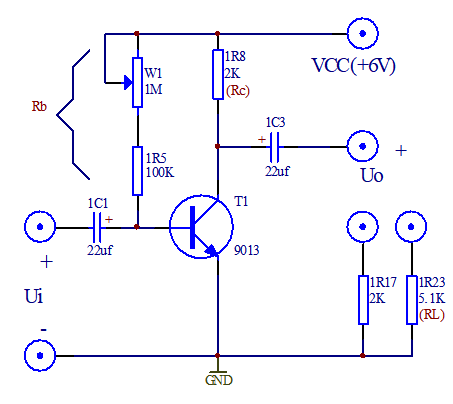
\includegraphics[width=0.4\linewidth]{电路图.png}
		\caption{实验电路图}
		\label{}
	\end{figure}
	$$
V_{cc} = 12 \, \mathrm{V} \quad 
U_c = 5.979 \, \mathrm{V} \quad 
U_B = 3.446 \, \mathrm{V} \quad 
U_E = 2.754 \, \mathrm{V} \quad 
R_B = 42.759 \,k\Omega $$\\$$
Rw1 = R_B - 20 k\Omega = 22.759 k\Omega \quad 
I_c = 2.509 \, \mathrm{mA} \quad 
I_B = 0.264 \, \mathrm{mA} \quad 
\beta = 9.5
$$

	\subsection{测量电压放大倍数及观察负载电阻对放大倍数的影响}
	在实验1的基础上,把输入对地断开,接入 f=1KHZ、U=5mV 的正弦波信号,负载电阻分别为 Ru=2K Ω、Ru=5.1KΩ 和 Re=∞,用毫伏表测量输出电压的值,用示波器观察输入电压和输出电压波形.
	\begin{center}
		\begin{tabular}{|c|c|c|c|}
		\hline
		$R_L$ & $U_i$ (mV) & $U_o$ (mV) & $A_u$ \\
		\hline
		2kΩ   & 1.775     & 10.691    & 6.023  \\
		5.1kΩ & 1.774     & 14.015    & 7.900  \\
		∞     & 1.775     & 17.131    & 9.651  \\
		\hline
		\end{tabular}
		\end{center}
		\subsection{测量输入电阻和输出电阻}	
		按图连好电路,测出电阻R1 两端对地信号电压 Ui及 U'。
		

\begin{figure}[{H}]
	\centering
	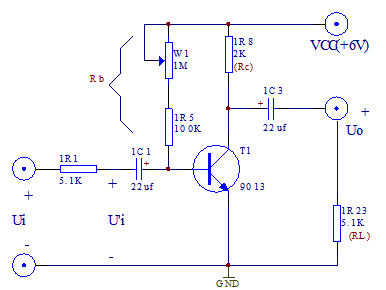
\includegraphics[width=0.4\linewidth]{电路图2.png}
	\caption{实验电路图}
	\label{}
\end{figure}
\begin{center}
			\begin{tabular}{|c|c|c|c|c|}
			\hline
			$U_i$ (mV) & $U_i'$ (mV) & $U_0$ (mV) & $U_\infty$ (mV) \\
			\hline
					0.415  & 1.819       & 19.06    & 27.13\\
			\hline
			\end{tabular}
			\end{center}
			\subsection{观察静态工作点对放大器输出波形的影响}		
\begin{figure}[{H}]
	\centering
	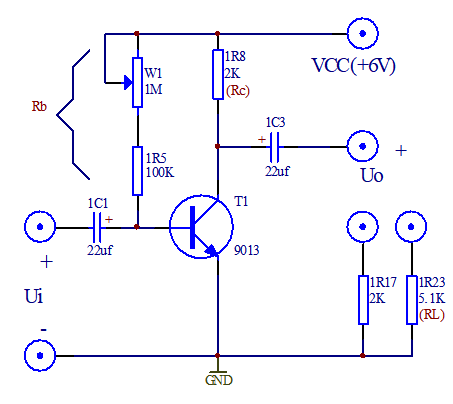
\includegraphics[width=0.4\linewidth]{电路图.png}
	\caption{实验电路图}
	\label{}
\end{figure}
\begin{enumerate}
    \item 输入端接入 $f = 1$ kHz、$U_i = 5$ mV 的正弦信号,用示波器观察正常工作时输出电压的波形,并将其描绘下来。
    \item 逐渐减小电位器 $W_1$ 的阻值,观察输出电压的变化。当输出电压波形出现明显削波失真时,描绘失真的波形,并说明是哪种失真。如果 $W_1 = 0$ Ω 后仍不出现失真,可以加大输入信号 $U_i$ 或将 $R_{B1}$ 从 100 kΩ 改为 10 kΩ,直到出现明显失真波形。
    \item 逐渐增大 $W_1$ 的阻值,观察输出电压的变化。当输出电压波形出现明显削波失真时,描绘失真的波形,并说明是哪种失真。如果 $W_1 = 1$ MΩ 后仍不出现失真,可以加大输入信号 $U_i$,直到出现明显失真波形。
    \item 调节 W1 使输出电压波形不失真且幅值为最大,测量此时的静态工作
	点 $U_{c}$, $U_{B}$, $R_{w}$和输出电压的数值。并估算此时的动态范围(用有效值表
	示)
\end{enumerate}
\begin{center}
	\begin{tabular}{|c|c|c|c|c|c|}
	\hline
	$U_i$ (mV) & $U_i'$ (mV) & $U_c$ (V) & $U_B$ (V) & $U_o$ (V) \\
	\hline
	100 & 253 & 4.683 & 4.085 & 0.483 \\
	\hline
	\end{tabular}
	\end{center}
	\begin{figure}[{H}]
		\centering
		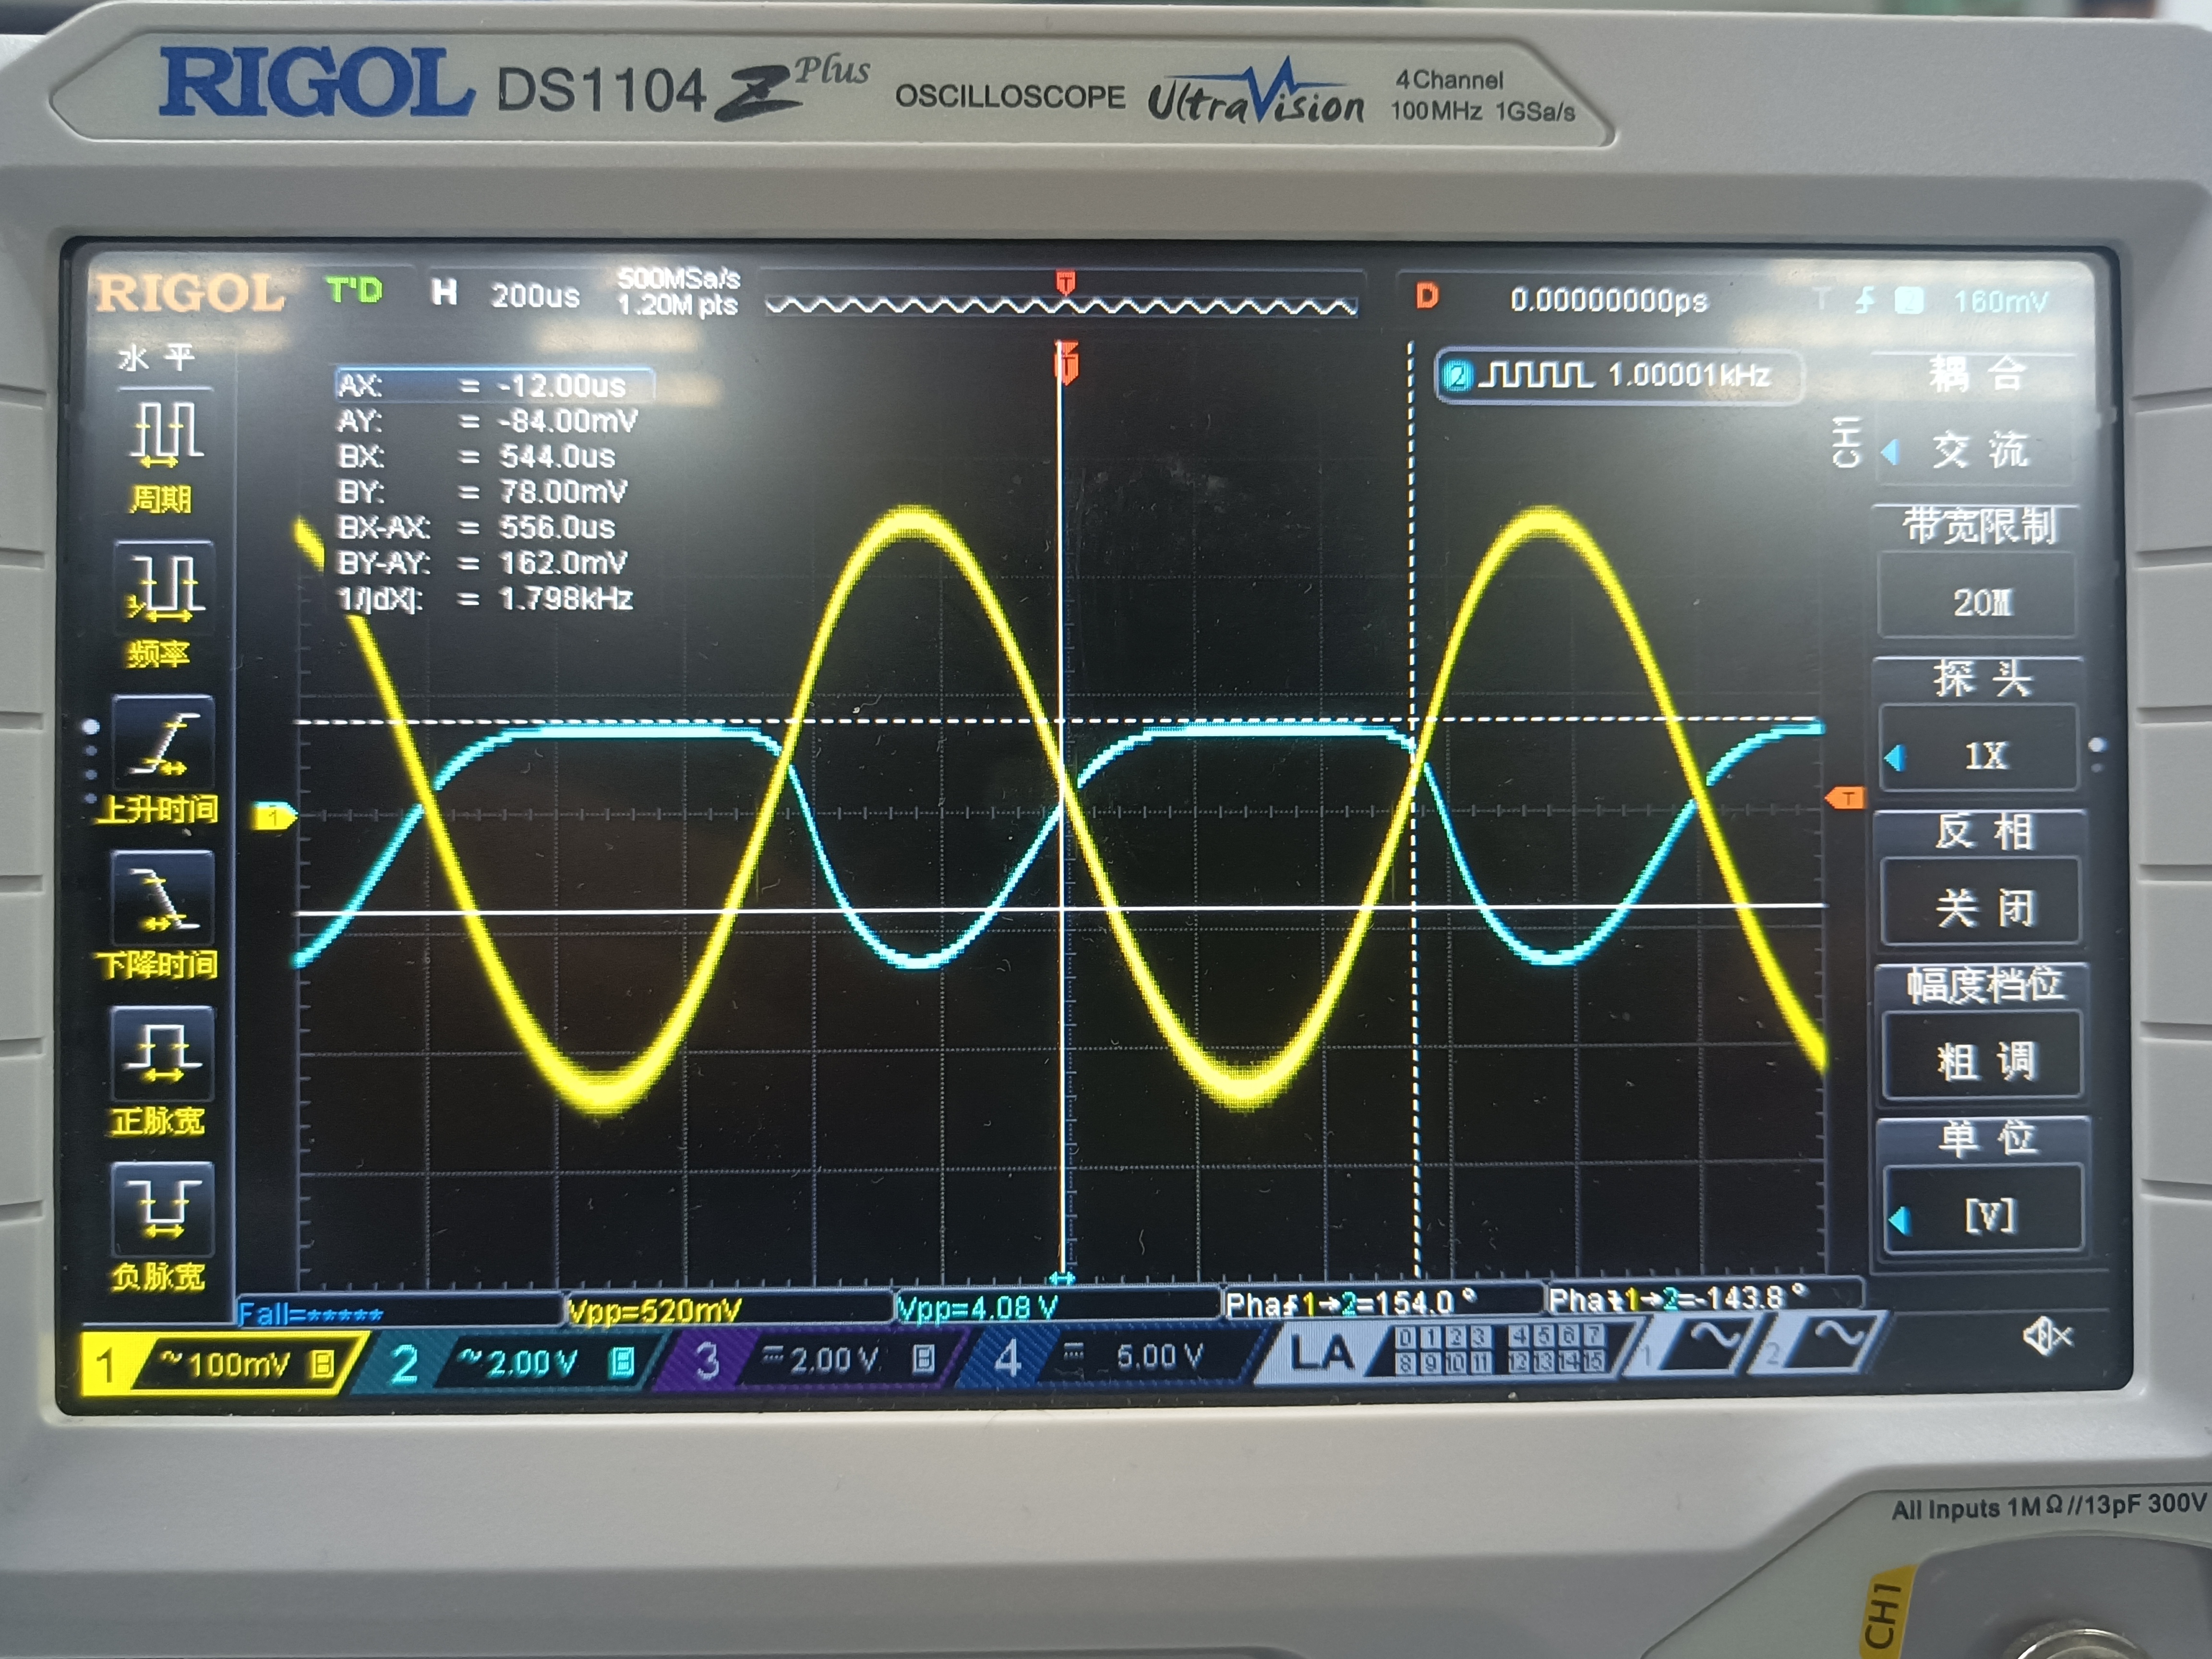
\includegraphics[width=0.45\linewidth]{失真.jpg}
		\caption{饱和失真}
		\label{}
	\end{figure}
	\begin{figure}[{H}]
		\centering
		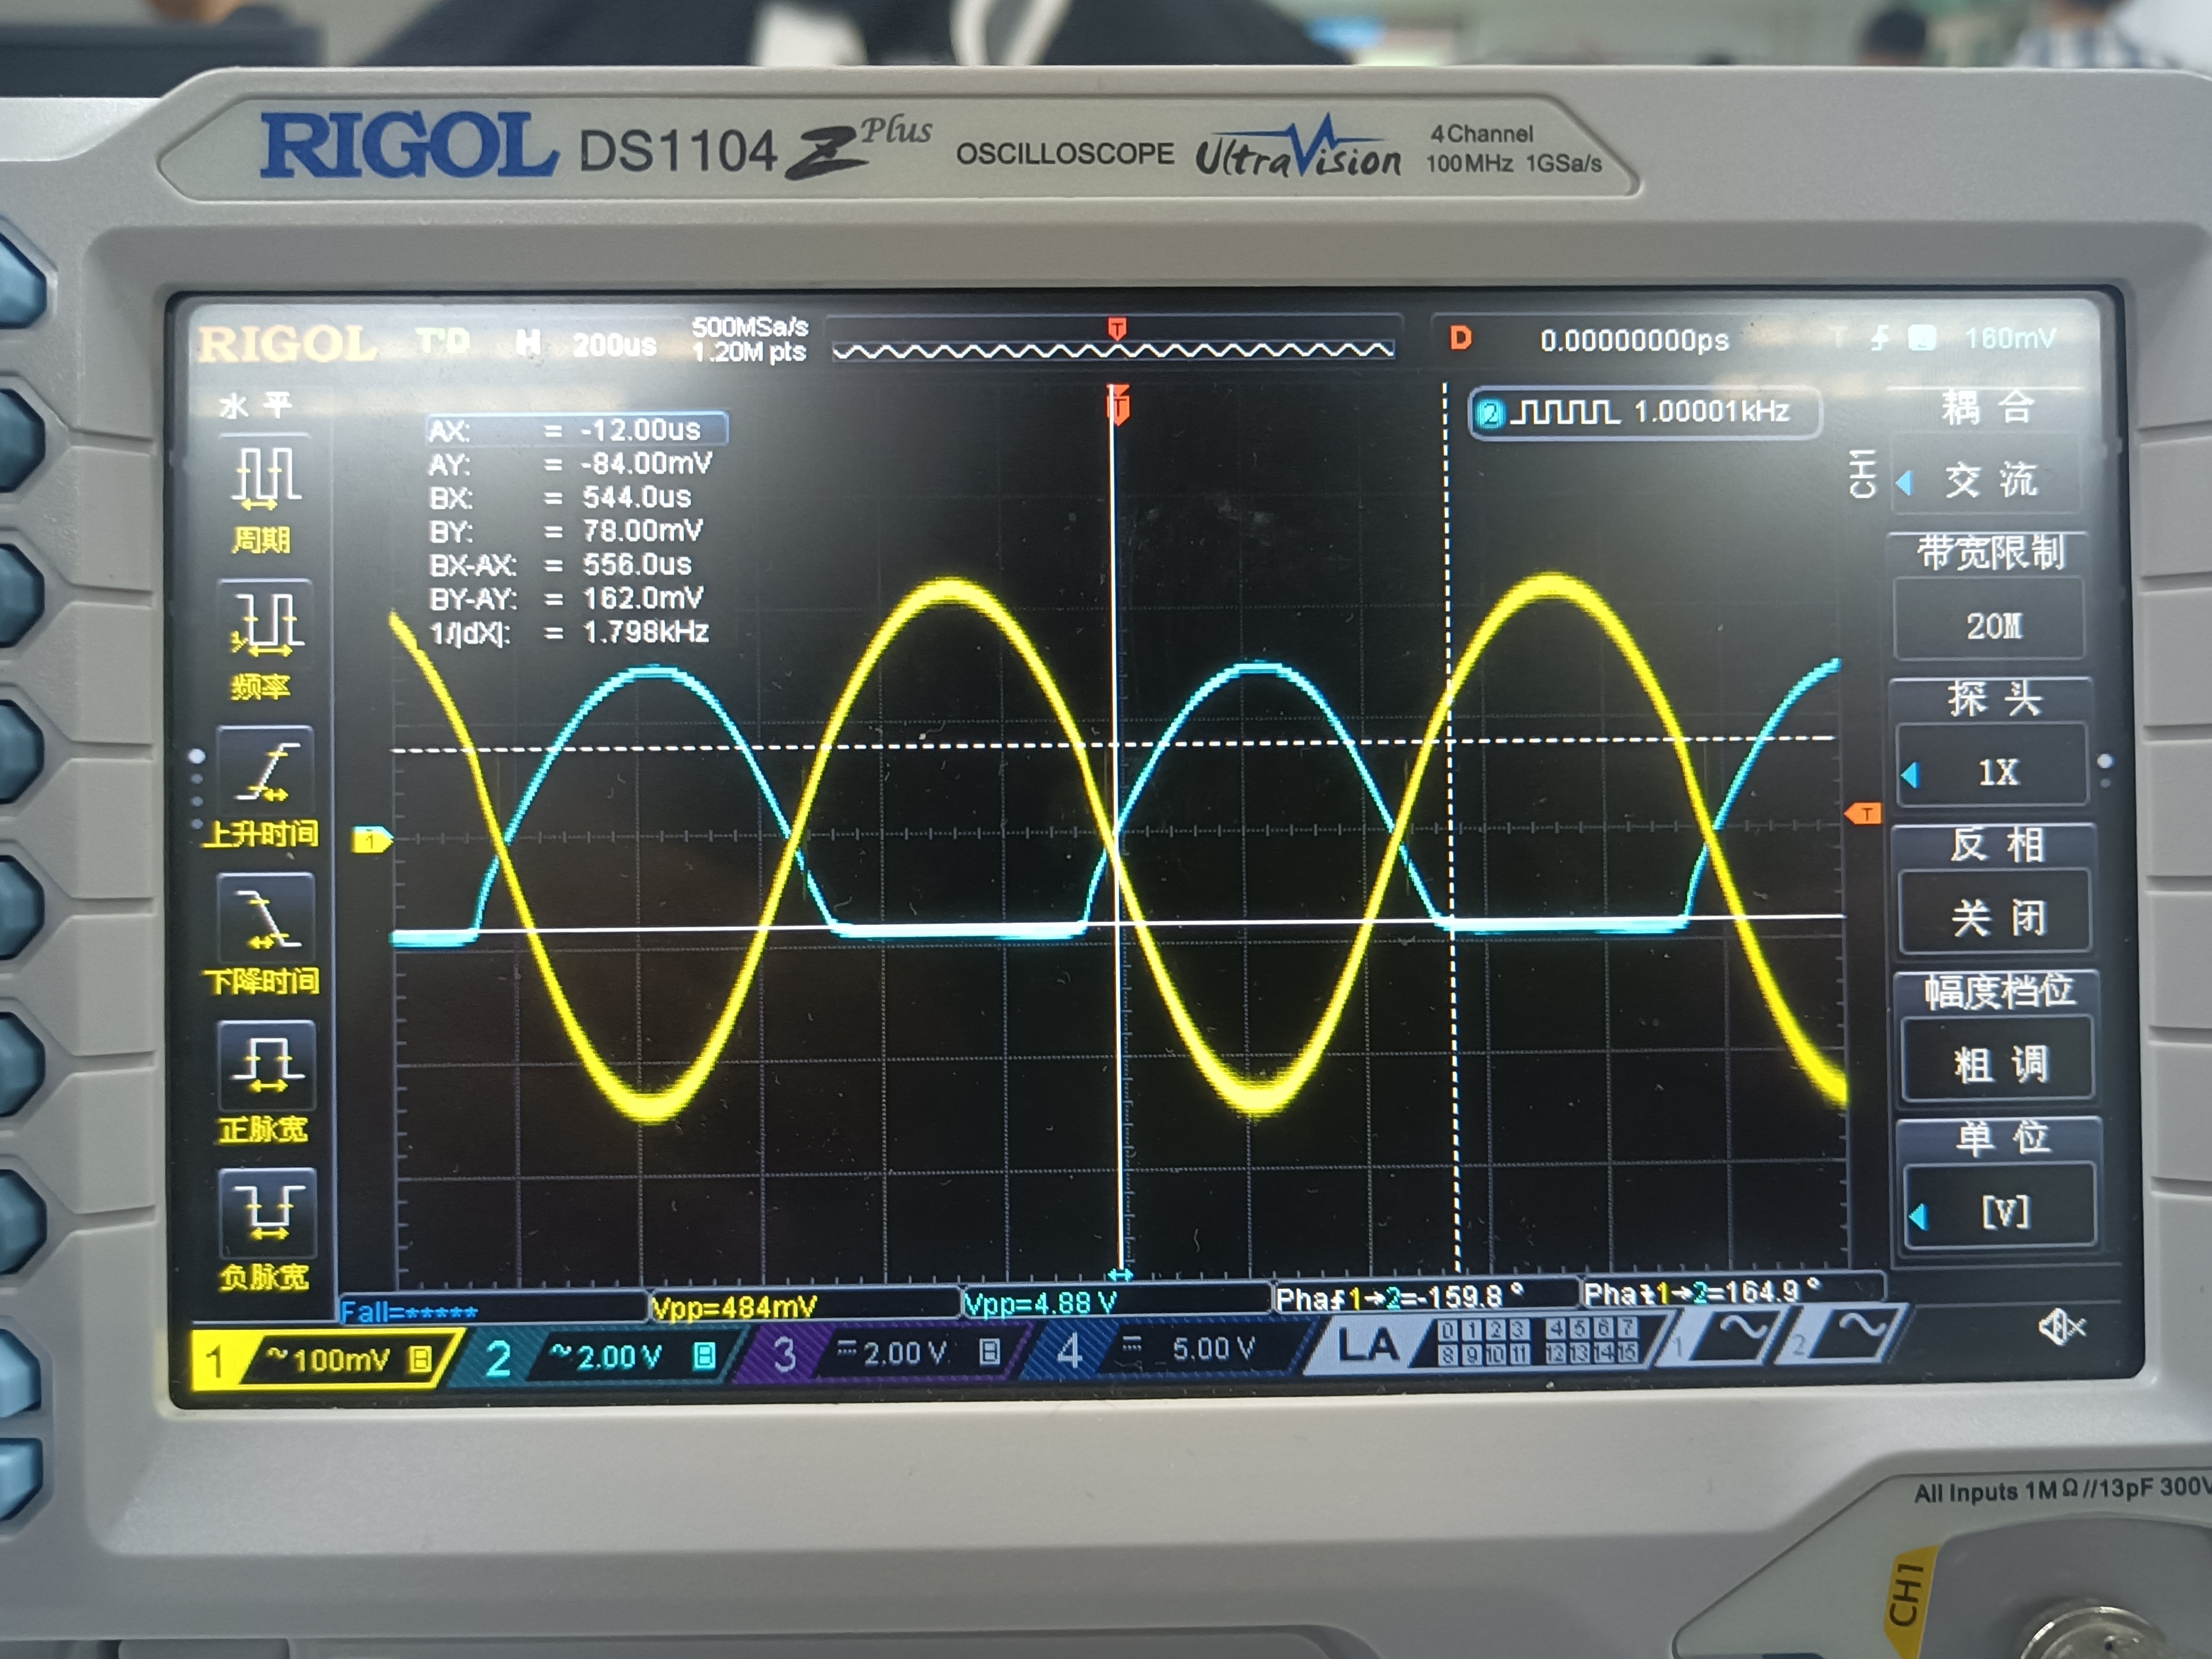
\includegraphics[width=0.45\linewidth]{失真2.jpg}
		\caption{截止失真}
		\label{}
	\end{figure}
	


	\clearpage
	
	\subsection{实验过程遇到问题及解决办法}
	\begin{enumerate}
		\item 实验中示波器一直无法稳定,在老师的帮助下将示波器的显示稳定下来后才得出了正确的实验图像。
		\item 实验中出现了接线的问题,需要较长的时间来完成接线,需要对于实验电路完全理解后才能完成。
	\end{enumerate}
	% ---
	
	
	
	% 分析与讨论	
	\clearpage
	
	% 顶栏
	\begin{table}
		\renewcommand\arraystretch{1.7}
		\begin{tabularx}{\textwidth}{|X|X|X|X|}
			\hline
			专业:& 物理学 &年级:& 2022级\\
			\hline
			姓名: &黄罗琳、王显  & 学号:& 22344001、22344002\\
			\hline
			日期:&  2024/4/24& 评分: &\\
			\hline
		\end{tabularx}
	\end{table}
	% ---
	
	% 小标题
	\section{ET8 单级交流放大器 \quad\heiti 分析与讨论}
	% ---
	
	% 数据处理
	\subsection{调节静态工作点}
	$$
V_{cc} = 12 \, \mathrm{V} \quad 
U_c = 5.979 \, \mathrm{V} \quad 
U_B = 3.446 \, \mathrm{V} \quad 
U_E = 2.754 \, \mathrm{V} \quad 
R_B = 42.759 \,k\Omega $$\\$$
Rw1 = R_B - 20 k\Omega = 22.759 k\Omega \quad 
I_c = 2.509 \, \mathrm{mA} \quad 
I_B = 0.264 \, \mathrm{mA} \quad 
\beta = 9.5
$$
	$$I_C=\frac{V_{CC}-U_C}{R_c}=2.509mA$$
	$$I_{B}=\frac{V_{CC}-U_{BE}}{R_{B}}=0.264m A$$
	此三极管放大倍数为$\beta = 9.5$
	%
	\subsection{测量输入电阻和输出电阻}
	$$R_i=\frac{U_i}{I_i}=\frac{U_i}{U_i^{'}-U_i}R=0.296k\Omega$$
	$$R_{o}=\frac{U_{\infty}-U_{OL}}{I_{o}}=\frac{U_{\infty}-U_{OL}}{U_{OL}}R_{L}=2.16k\Omega$$
	%
	\subsection{观察静态工作点对放大器输出波形的影响}
	\begin{center}
		\begin{tabular}{|c|c|c|c|c|c|}
		\hline
		$U_i$ (mV) & $U_i'$ (mV) & $U_c$ (V) & $U_B$ (V) & $U_o$ (V) \\
		\hline
		100 & 253 & 4.683 & 4.085 & 0.483 \\
		\hline
		\end{tabular}
		\end{center}
	动态范围为1.443V-1.726V

	削波是放大器输出波形被“削去”的现象,这通常发生在放大器的三极管工作在截止或饱和状态时。削波导致输出信号的波形失真。


在放大器中,截止状态是指三极管等有源器件处于非导通状态,导致电流无法通过。当输入信号的负半周期使放大器进入截止状态时,输出信号无法继续复制负峰值的部分。结果,输出信号的波形被截断,导致削波。

\textbf{如图6的下半部分被截断}

饱和状态是指三极管等有源器件达到最大导通程度,无法进一步增加电流。当输入信号的正半周期使放大器进入饱和状态时,输出信号的正峰值部分被限制在某个固定值。这样,输出信号也会被剪掉,导致削波。

\textbf{如图5的上半部分被截断}


	
	\subsection{实验思考题}
	
	%思考题1
	\begin{question}
		实验电路的参数$R_L$及$V_CC$变化,对输出信号的动态范围有何影响?如果输入信号加大,输出信号的波形将产生什么失真?
	\end{question}
	$R_L$减小会使放大倍数下降,但加大输入后动态范围不变。若$V_{cc}$增大,输出信号的动态范围会加大。\\
如果输出信号幅值过大,则输出信号波形既会存在饱和失真又会存在截止失真,输出图像为输出波形上下两端都将变平。
	% 思考题2
	\begin{question}
		本实验在测量放大器放大倍数时,使用交流毫伏表,而不用万用表,为什么?
	\end{question}
	交流毫伏表的阻抗极大,对实验影响可忽略不计,而万用表的阻抗为几千欧(较小),对于放大电路来说不可忽略,使得输出电压测量不准确。

此外,交流毫伏表的测量参数会比万用表大,更加适配此实验。
	% 思考题3
	\begin{question}
		测一个放大器的输入电阻时,若选取的串入电阻过大或过小,则会出现测试误差,请分析测试误差。
	\end{question}
	输入电阻测量公式为:
$$R_i=\frac{U_i}{I_i}=\frac{U_i}{U_i^{\prime}-U_i}R$$

···若串入电阻$R$过大,则根据分压公式$U_i=\frac{R_i}{R+R_i}U_i^{\prime}$,所测得$U_\mathrm{i}$值会很低,误差可能较大,会导致输入电阻$R_i$测量不准确。

···若串入电阻$R$过小,则$U_i^\prime$与$U_i$近似相等,无法计算输入电阻$R_i.$
	% ---
	
	
	% 结语部分
	\clearpage
	
	% 小标题
	\section{ET8 单级交流放大器\quad\heiti 结语}
	% ---
	
	% 总结、杂谈与致谢
	\subsection{实验心得和体会、意见建议等}
	\begin{enumerate}
		\item 实验总体难度体现在接线,若能完成正确的线路,则可以充分理解实验目的和原理。
		\item 此实验能够深入了解放大器的工作原理和方式,为进一步学习打下基础。
		\item \textbf{本实验报告采用LATEX编辑,实验分工为黄罗琳同学负责记录数据、编辑报告、数据分析,王显同学负责实验操作、误差分析、数据绘图。}
	\end{enumerate}
	\quad \large \textbf{感谢您对于此篇实验报告的阅读与批改,祝您工作顺利!}
	% ---
	

	% 附件
	\subsection{附件}
	\begin{figure}[H]
		\centering
		\begin{minipage}[t]{0.45\textwidth}
			\centering
			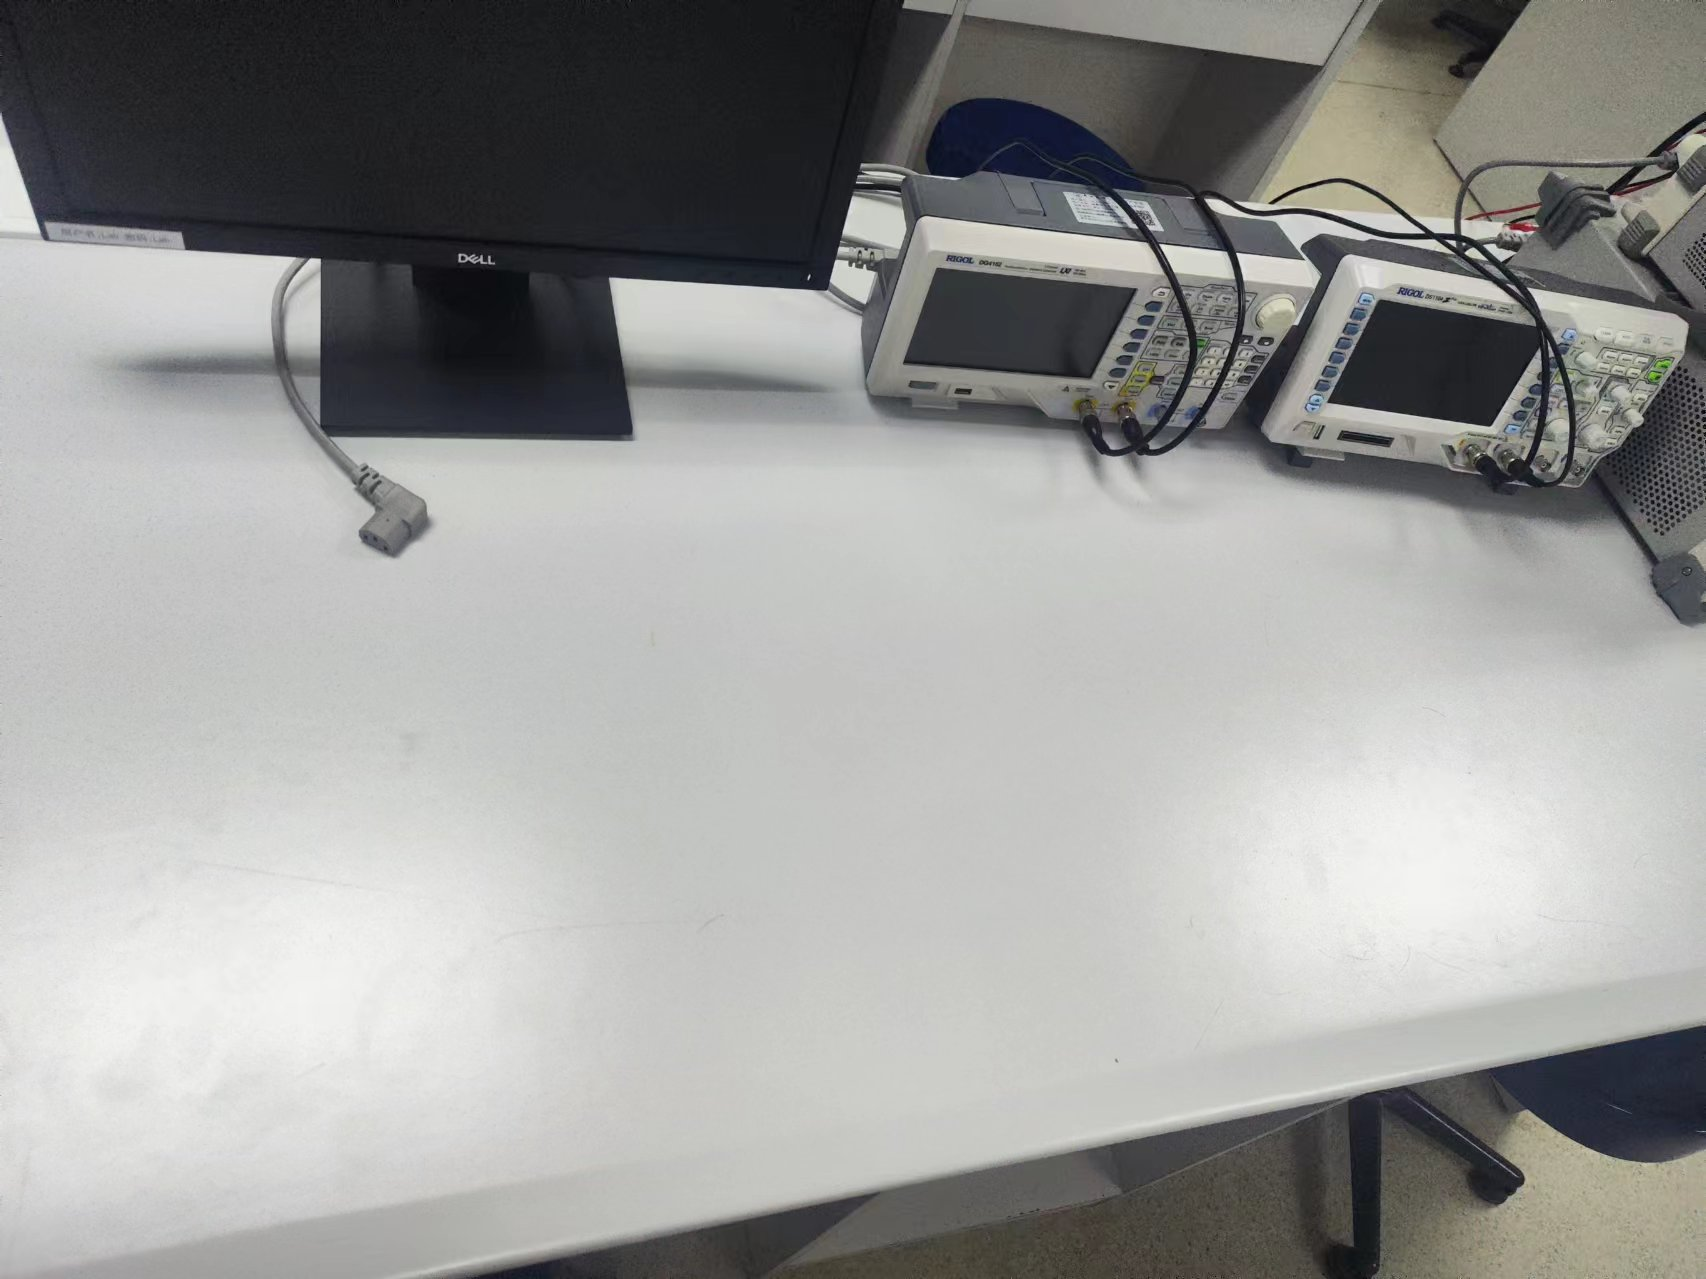
\includegraphics[width=0.8\linewidth]{桌面.jpg}
			\caption{实验桌面整理}
		\end{minipage}
		\hfill % 或使用 \quad 或 \hspace{5mm} 来控制间距
		\begin{minipage}[t]{0.45\textwidth}
			\centering
			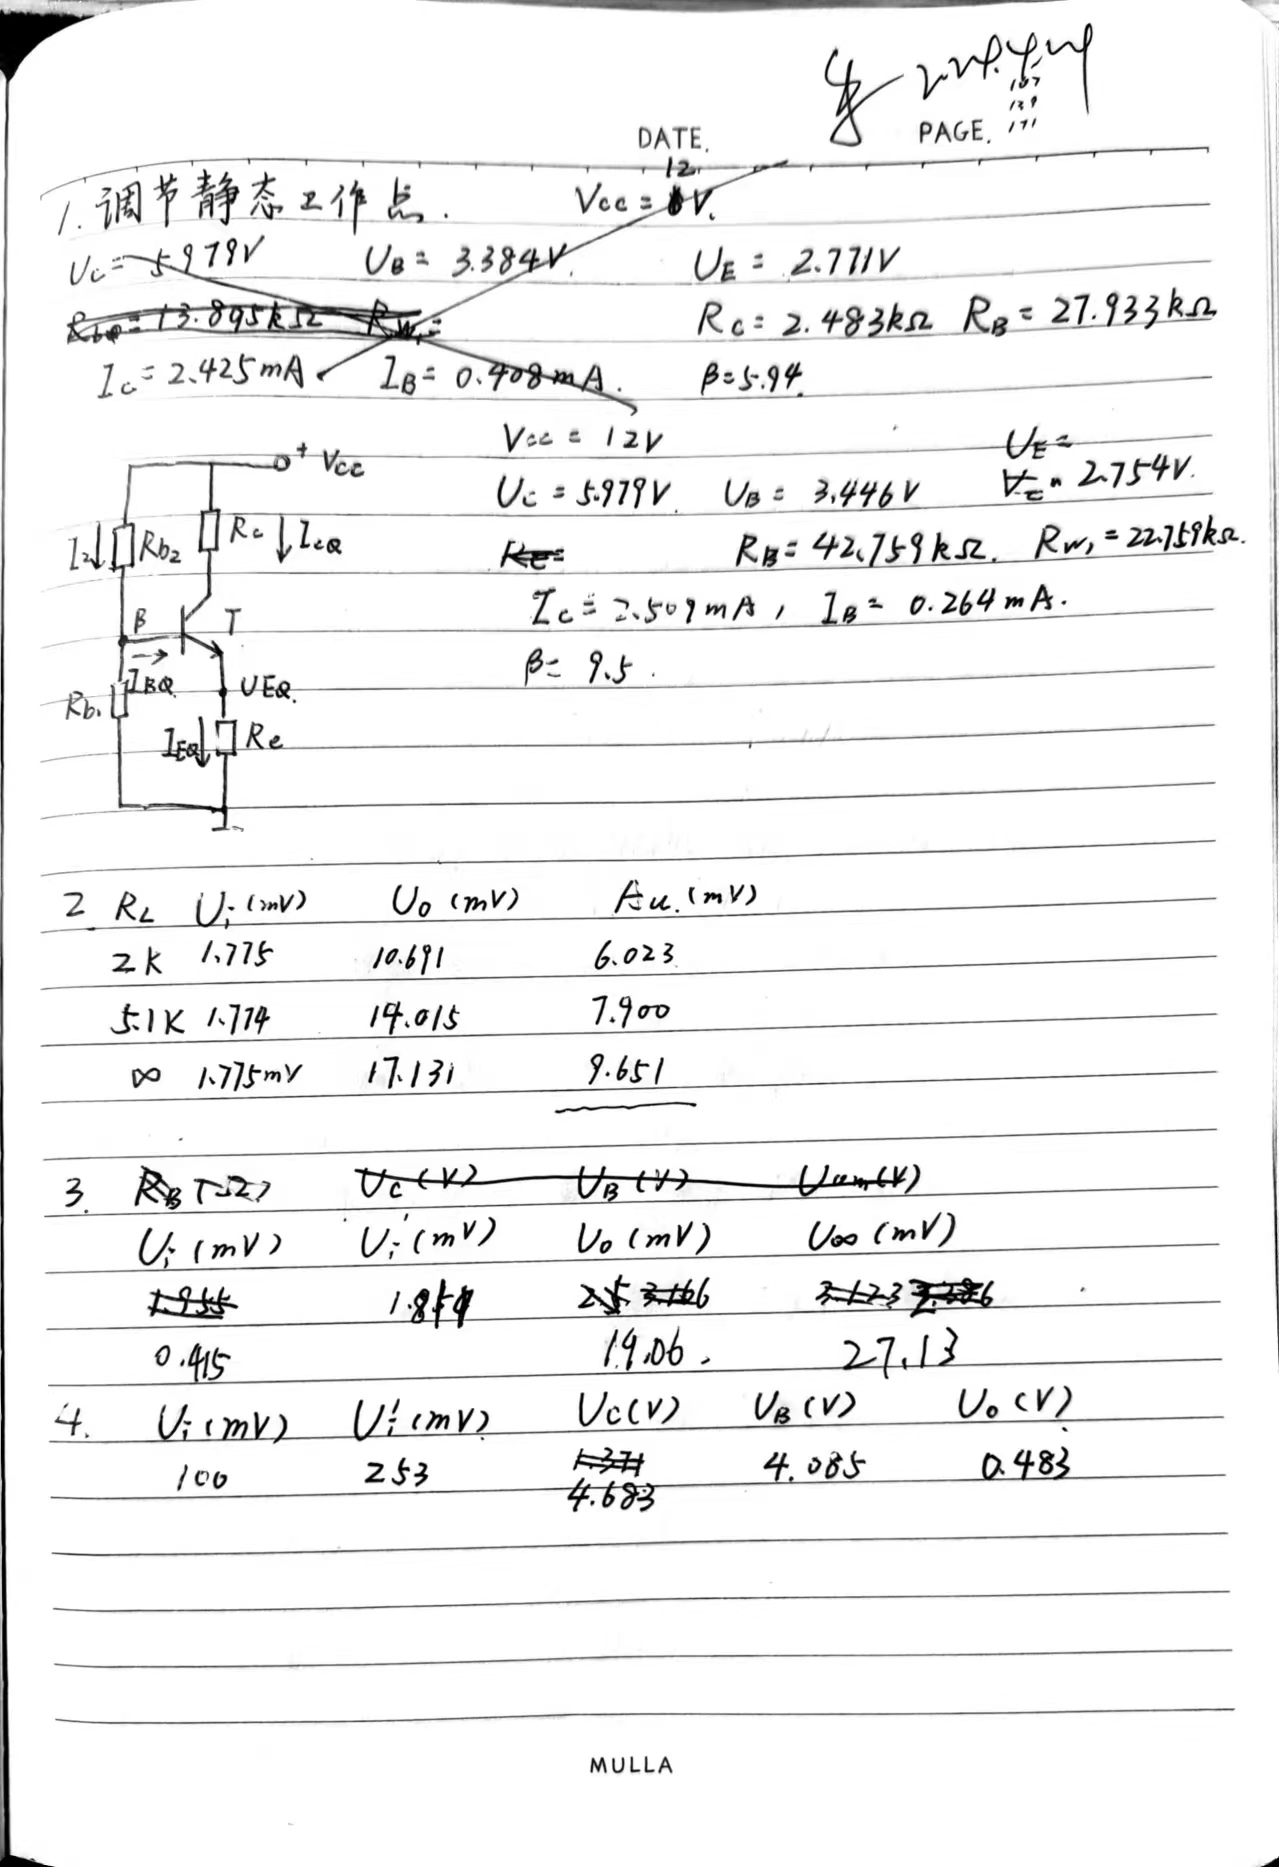
\includegraphics[width=0.5\linewidth]{实验数据.jpg}
			\caption{实验数据}
		\end{minipage}
	\end{figure}
	% ---
	
	
\end{document}